\documentclass[1p]{elsarticle_modified}
%\bibliographystyle{elsarticle-num}

%\usepackage[colorlinks]{hyperref}
%\usepackage{abbrmath_seonhwa} %\Abb, \Ascr, \Acal ,\Abf, \Afrak
\usepackage{amsfonts}
\usepackage{amssymb}
\usepackage{amsmath}
\usepackage{amsthm}
\usepackage{scalefnt}
\usepackage{amsbsy}
\usepackage{kotex}
\usepackage{caption}
\usepackage{subfig}
\usepackage{color}
\usepackage{graphicx}
\usepackage{xcolor} %% white, black, red, green, blue, cyan, magenta, yellow
\usepackage{float}
\usepackage{setspace}
\usepackage{hyperref}

\usepackage{tikz}
\usetikzlibrary{arrows}

\usepackage{multirow}
\usepackage{array} % fixed length table
\usepackage{hhline}

%%%%%%%%%%%%%%%%%%%%%
\makeatletter
\renewcommand*\env@matrix[1][\arraystretch]{%
	\edef\arraystretch{#1}%
	\hskip -\arraycolsep
	\let\@ifnextchar\new@ifnextchar
	\array{*\c@MaxMatrixCols c}}
\makeatother %https://tex.stackexchange.com/questions/14071/how-can-i-increase-the-line-spacing-in-a-matrix
%%%%%%%%%%%%%%%

\usepackage[normalem]{ulem}

\newcommand{\msout}[1]{\ifmmode\text{\sout{\ensuremath{#1}}}\else\sout{#1}\fi}
%SOURCE: \msout is \stkout macro in https://tex.stackexchange.com/questions/20609/strikeout-in-math-mode

\newcommand{\cancel}[1]{
	\ifmmode
	{\color{red}\msout{#1}}
	\else
	{\color{red}\sout{#1}}
	\fi
}

\newcommand{\add}[1]{
	{\color{blue}\uwave{#1}}
}

\newcommand{\replace}[2]{
	\ifmmode
	{\color{red}\msout{#1}}{\color{blue}\uwave{#2}}
	\else
	{\color{red}\sout{#1}}{\color{blue}\uwave{#2}}
	\fi
}

\newcommand{\Sol}{\mathcal{S}} %segment
\newcommand{\D}{D} %diagram
\newcommand{\A}{\mathcal{A}} %arc


%%%%%%%%%%%%%%%%%%%%%%%%%%%%%5 test

\def\sl{\operatorname{\textup{SL}}(2,\Cbb)}
\def\psl{\operatorname{\textup{PSL}}(2,\Cbb)}
\def\quan{\mkern 1mu \triangleright \mkern 1mu}

\theoremstyle{definition}
\newtheorem{thm}{Theorem}[section]
\newtheorem{prop}[thm]{Proposition}
\newtheorem{lem}[thm]{Lemma}
\newtheorem{ques}[thm]{Question}
\newtheorem{cor}[thm]{Corollary}
\newtheorem{defn}[thm]{Definition}
\newtheorem{exam}[thm]{Example}
\newtheorem{rmk}[thm]{Remark}
\newtheorem{alg}[thm]{Algorithm}

\newcommand{\I}{\sqrt{-1}}
\begin{document}

%\begin{frontmatter}
%
%\title{Boundary parabolic representations of knots up to 8 crossings}
%
%%% Group authors per affiliation:
%\author{Yunhi Cho} 
%\address{Department of Mathematics, University of Seoul, Seoul, Korea}
%\ead{yhcho@uos.ac.kr}
%
%
%\author{Seonhwa Kim} %\fnref{s_kim}}
%\address{Center for Geometry and Physics, Institute for Basic Science, Pohang, 37673, Korea}
%\ead{ryeona17@ibs.re.kr}
%
%\author{Hyuk Kim}
%\address{Department of Mathematical Sciences, Seoul National University, Seoul 08826, Korea}
%\ead{hyukkim@snu.ac.kr}
%
%\author{Seokbeom Yoon}
%\address{Department of Mathematical Sciences, Seoul National University, Seoul, 08826,  Korea}
%\ead{sbyoon15@snu.ac.kr}
%
%\begin{abstract}
%We find all boundary parabolic representation of knots up to 8 crossings.
%
%\end{abstract}
%\begin{keyword}
%    \MSC[2010] 57M25 
%\end{keyword}
%
%\end{frontmatter}

%\linenumbers
%\tableofcontents
%
\newcommand\colored[1]{\textcolor{white}{\rule[-0.35ex]{0.8em}{1.4ex}}\kern-0.8em\color{red} #1}%
%\newcommand\colored[1]{\textcolor{white}{ #1}\kern-2.17ex	\textcolor{white}{ #1}\kern-1.81ex	\textcolor{white}{ #1}\kern-2.15ex\color{red}#1	}

{\Large $\underline{11a_{50}~(K11a_{50})}$}

\setlength{\tabcolsep}{10pt}
\renewcommand{\arraystretch}{1.6}
\vspace{1cm}\begin{tabular}{m{100pt}>{\centering\arraybackslash}m{274pt}}
\multirow{5}{120pt}{
	\centering
	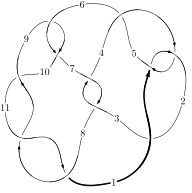
\includegraphics[width=112pt]{../../../GIT/diagram.site/Diagrams/png/299_11a_50.png}\\
\ \ \ A knot diagram\footnotemark}&
\allowdisplaybreaks
\textbf{Linearized knot diagam} \\
\cline{2-2}
 &
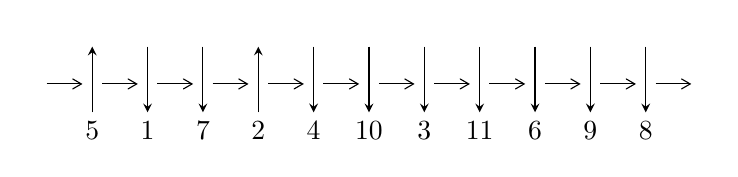
\begin{tikzpicture}[x=20pt, y=17pt]
	% nodes
	\node (C0) at (0, 0) {};
	\node (C1) at (1, 0) {};
	\node (C1U) at (1, +1) {};
	\node (C1D) at (1, -1) {5};

	\node (C2) at (2, 0) {};
	\node (C2U) at (2, +1) {};
	\node (C2D) at (2, -1) {1};

	\node (C3) at (3, 0) {};
	\node (C3U) at (3, +1) {};
	\node (C3D) at (3, -1) {7};

	\node (C4) at (4, 0) {};
	\node (C4U) at (4, +1) {};
	\node (C4D) at (4, -1) {2};

	\node (C5) at (5, 0) {};
	\node (C5U) at (5, +1) {};
	\node (C5D) at (5, -1) {4};

	\node (C6) at (6, 0) {};
	\node (C6U) at (6, +1) {};
	\node (C6D) at (6, -1) {10};

	\node (C7) at (7, 0) {};
	\node (C7U) at (7, +1) {};
	\node (C7D) at (7, -1) {3};

	\node (C8) at (8, 0) {};
	\node (C8U) at (8, +1) {};
	\node (C8D) at (8, -1) {11};

	\node (C9) at (9, 0) {};
	\node (C9U) at (9, +1) {};
	\node (C9D) at (9, -1) {6};

	\node (C10) at (10, 0) {};
	\node (C10U) at (10, +1) {};
	\node (C10D) at (10, -1) {9};

	\node (C11) at (11, 0) {};
	\node (C11U) at (11, +1) {};
	\node (C11D) at (11, -1) {8};
	\node (C12) at (12, 0) {};

	% arrows
	\draw[->,>={angle 60}]
	(C0) edge (C1) (C1) edge (C2) (C2) edge (C3) (C3) edge (C4) (C4) edge (C5) (C5) edge (C6) (C6) edge (C7) (C7) edge (C8) (C8) edge (C9) (C9) edge (C10) (C10) edge (C11) (C11) edge (C12) ;	\draw[->,>=stealth]
	(C1D) edge (C1U) (C2U) edge (C2D) (C3U) edge (C3D) (C4D) edge (C4U) (C5U) edge (C5D) (C6U) edge (C6D) (C7U) edge (C7D) (C8U) edge (C8D) (C9U) edge (C9D) (C10U) edge (C10D) (C11U) edge (C11D) ;
	\end{tikzpicture} \\
\hhline{~~} \\& 
\textbf{Solving Sequence} \\ \cline{2-2} 
 &
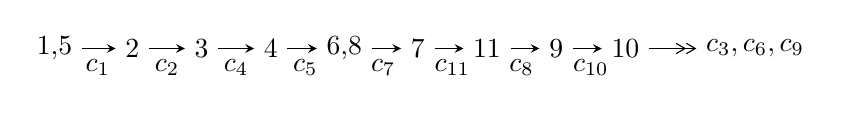
\begin{tikzpicture}[x=25pt, y=7pt]
	% node
	\node (A0) at (-1/8, 0) {1,5};
	\node (A1) at (1, 0) {2};
	\node (A2) at (2, 0) {3};
	\node (A3) at (3, 0) {4};
	\node (A4) at (65/16, 0) {6,8};
	\node (A5) at (41/8, 0) {7};
	\node (A6) at (49/8, 0) {11};
	\node (A7) at (57/8, 0) {9};
	\node (A8) at (65/8, 0) {10};
	\node (C1) at (1/2, -1) {$c_{1}$};
	\node (C2) at (3/2, -1) {$c_{2}$};
	\node (C3) at (5/2, -1) {$c_{4}$};
	\node (C4) at (7/2, -1) {$c_{5}$};
	\node (C5) at (37/8, -1) {$c_{7}$};
	\node (C6) at (45/8, -1) {$c_{11}$};
	\node (C7) at (53/8, -1) {$c_{8}$};
	\node (C8) at (61/8, -1) {$c_{10}$};
	\node (A9) at (10, 0) {$c_{3},c_{6},c_{9}$};

	% edge
	\draw[->,>=stealth]	
	(A0) edge (A1) (A1) edge (A2) (A2) edge (A3) (A3) edge (A4) (A4) edge (A5) (A5) edge (A6) (A6) edge (A7) (A7) edge (A8) ;
	\draw[->>,>={angle 60}]	
	(A8) edge (A9);
\end{tikzpicture} \\ 

\end{tabular} \\

\footnotetext{
The image of knot diagram is generated by the software ``\textbf{Draw programme}" developed by Andrew Bartholomew(\url{http://www.layer8.co.uk/maths/draw/index.htm\#Running-draw}), where we modified some parts for our purpose(\url{https://github.com/CATsTAILs/LinksPainter}).
}\phantom \\ \newline 
\centering \textbf{Ideals for irreducible components\footnotemark of $X_{\text{par}}$} 
 
\begin{align*}
I^u_{1}&=\langle 
-2 u^{46}+9 u^{45}+\cdots+4 b+5,\;- u^{46}+18 u^{45}+\cdots+4 a-25,\;u^{47}-4 u^{46}+\cdots+6 u-1\rangle \\
I^u_{2}&=\langle 
- a u+b,\;a^3- a^2 u- a^2+2 a u+1,\;u^2+u+1\rangle \\
\\
\end{align*}
\raggedright * 2 irreducible components of $\dim_{\mathbb{C}}=0$, with total 53 representations.\\
\footnotetext{All coefficients of polynomials are rational numbers. But the coefficients are sometimes approximated in decimal forms when there is not enough margin.}
\newpage
\renewcommand{\arraystretch}{1}
\centering \section*{I. $I^u_{1}= \langle -2 u^{46}+9 u^{45}+\cdots+4 b+5,\;- u^{46}+18 u^{45}+\cdots+4 a-25,\;u^{47}-4 u^{46}+\cdots+6 u-1 \rangle$}
\flushleft \textbf{(i) Arc colorings}\\
\begin{tabular}{m{7pt} m{180pt} m{7pt} m{180pt} }
\flushright $a_{1}=$&$\begin{pmatrix}1\\0\end{pmatrix}$ \\
\flushright $a_{5}=$&$\begin{pmatrix}0\\u\end{pmatrix}$ \\
\flushright $a_{2}=$&$\begin{pmatrix}1\\- u^2\end{pmatrix}$ \\
\flushright $a_{3}=$&$\begin{pmatrix}u^2+1\\- u^2\end{pmatrix}$ \\
\flushright $a_{4}=$&$\begin{pmatrix}- u\\u^3+u\end{pmatrix}$ \\
\flushright $a_{6}=$&$\begin{pmatrix}- u^3\\u^5+u^3+u\end{pmatrix}$ \\
\flushright $a_{8}=$&$\begin{pmatrix}\frac{1}{4} u^{46}-\frac{9}{2} u^{45}+\cdots-17 u+\frac{25}{4}\\\frac{1}{2} u^{46}-\frac{9}{4} u^{45}+\cdots+\frac{9}{4} u-\frac{5}{4}\end{pmatrix}$ \\
\flushright $a_{7}=$&$\begin{pmatrix}\frac{7}{4} u^{46}-\frac{5}{2} u^{45}+\cdots+2 u+\frac{7}{4}\\-\frac{9}{2} u^{46}+\frac{41}{4} u^{45}+\cdots+\frac{35}{4} u-\frac{7}{4}\end{pmatrix}$ \\
\flushright $a_{11}=$&$\begin{pmatrix}-\frac{1}{4} u^{46}+\frac{3}{4} u^{45}+\cdots+\frac{13}{4} u+2\\\frac{1}{4} u^{46}- u^{45}+\cdots-\frac{5}{2} u+\frac{1}{4}\end{pmatrix}$ \\
\flushright $a_{9}=$&$\begin{pmatrix}-2 u^{46}+\frac{15}{2} u^{45}+\cdots+20 u+1\\-\frac{5}{4} u^{46}+\frac{13}{4} u^{45}+\cdots-\frac{11}{4} u+\frac{1}{2}\end{pmatrix}$ \\
\flushright $a_{10}=$&$\begin{pmatrix}-\frac{7}{4} u^{46}+\frac{33}{4} u^{45}+\cdots+\frac{107}{4} u-\frac{1}{2}\\-\frac{5}{4} u^{46}+\frac{9}{4} u^{45}+\cdots-\frac{31}{4} u+\frac{3}{2}\end{pmatrix}$\\ \flushright $a_{10}=$&$\begin{pmatrix}-\frac{7}{4} u^{46}+\frac{33}{4} u^{45}+\cdots+\frac{107}{4} u-\frac{1}{2}\\-\frac{5}{4} u^{46}+\frac{9}{4} u^{45}+\cdots-\frac{31}{4} u+\frac{3}{2}\end{pmatrix}$\\&\end{tabular}
\flushleft \textbf{(ii) Obstruction class $= -1$}\\~\\
\flushleft \textbf{(iii) Cusp Shapes $= -9 u^{46}+\frac{33}{2} u^{45}+\cdots-27 u-4$}\\~\\
\newpage\renewcommand{\arraystretch}{1}
\flushleft \textbf{(iv) u-Polynomials at the component}\newline \\
\begin{tabular}{m{50pt}|m{274pt}}
Crossings & \hspace{64pt}u-Polynomials at each crossing \\
\hline $$\begin{aligned}c_{1},c_{4}\end{aligned}$$&$\begin{aligned}
&u^{47}+4 u^{46}+\cdots+6 u+1
\end{aligned}$\\
\hline $$\begin{aligned}c_{2},c_{5}\end{aligned}$$&$\begin{aligned}
&u^{47}+14 u^{46}+\cdots+38 u-1
\end{aligned}$\\
\hline $$\begin{aligned}c_{3},c_{7}\end{aligned}$$&$\begin{aligned}
&u^{47}- u^{46}+\cdots+96 u+64
\end{aligned}$\\
\hline $$\begin{aligned}c_{6},c_{9}\end{aligned}$$&$\begin{aligned}
&u^{47}+3 u^{46}+\cdots- u+1
\end{aligned}$\\
\hline $$\begin{aligned}c_{8},c_{10},c_{11}\end{aligned}$$&$\begin{aligned}
&u^{47}+11 u^{46}+\cdots+u+1
\end{aligned}$\\
\hline
\end{tabular}\\~\\
\newpage\renewcommand{\arraystretch}{1}
\flushleft \textbf{(v) Riley Polynomials at the component}\newline \\
\begin{tabular}{m{50pt}|m{274pt}}
Crossings & \hspace{64pt}Riley Polynomials at each crossing \\
\hline $$\begin{aligned}c_{1},c_{4}\end{aligned}$$&$\begin{aligned}
&y^{47}+14 y^{46}+\cdots+38 y-1
\end{aligned}$\\
\hline $$\begin{aligned}c_{2},c_{5}\end{aligned}$$&$\begin{aligned}
&y^{47}+42 y^{46}+\cdots+2346 y-1
\end{aligned}$\\
\hline $$\begin{aligned}c_{3},c_{7}\end{aligned}$$&$\begin{aligned}
&y^{47}+35 y^{46}+\cdots-23552 y-4096
\end{aligned}$\\
\hline $$\begin{aligned}c_{6},c_{9}\end{aligned}$$&$\begin{aligned}
&y^{47}-11 y^{46}+\cdots+y-1
\end{aligned}$\\
\hline $$\begin{aligned}c_{8},c_{10},c_{11}\end{aligned}$$&$\begin{aligned}
&y^{47}+53 y^{46}+\cdots+41 y-1
\end{aligned}$\\
\hline
\end{tabular}\\~\\
\newpage\flushleft \textbf{(vi) Complex Volumes and Cusp Shapes}
$$\begin{array}{c|c|c}  
\text{Solutions to }I^u_{1}& \I (\text{vol} + \sqrt{-1}CS) & \text{Cusp shape}\\
 \hline 
\begin{aligned}
u &= -0.663428 + 0.780790 I \\
a &= \phantom{-}1.00646 - 1.05901 I \\
b &= -0.205400 + 0.577345 I\end{aligned}
 & \phantom{-}1.047100 - 0.807076 I & -4.48198 - 0.15159 I \\ \hline\begin{aligned}
u &= -0.663428 - 0.780790 I \\
a &= \phantom{-}1.00646 + 1.05901 I \\
b &= -0.205400 - 0.577345 I\end{aligned}
 & \phantom{-}1.047100 + 0.807076 I & -4.48198 + 0.15159 I \\ \hline\begin{aligned}
u &= -0.199822 + 1.009780 I \\
a &= -0.834043 - 0.291155 I \\
b &= -0.625995 - 0.626906 I\end{aligned}
 & -2.01497 - 4.25844 I & -10.22284 + 8.38293 I \\ \hline\begin{aligned}
u &= -0.199822 - 1.009780 I \\
a &= -0.834043 + 0.291155 I \\
b &= -0.625995 + 0.626906 I\end{aligned}
 & -2.01497 + 4.25844 I & -10.22284 - 8.38293 I \\ \hline\begin{aligned}
u &= -0.461388 + 0.956277 I \\
a &= \phantom{-}0.665200 + 0.526100 I \\
b &= -0.316069 + 0.253513 I\end{aligned}
 & -0.63663 - 1.64887 I & -2.14725 - 2.29266 I \\ \hline\begin{aligned}
u &= -0.461388 - 0.956277 I \\
a &= \phantom{-}0.665200 - 0.526100 I \\
b &= -0.316069 - 0.253513 I\end{aligned}
 & -0.63663 + 1.64887 I & -2.14725 + 2.29266 I \\ \hline\begin{aligned}
u &= \phantom{-}0.810606 + 0.776375 I \\
a &= \phantom{-}0.565835 + 0.632629 I \\
b &= -0.750225 - 1.009350 I\end{aligned}
 & \phantom{-}4.58669 - 3.21526 I & -3.05328 + 3.33895 I \\ \hline\begin{aligned}
u &= \phantom{-}0.810606 - 0.776375 I \\
a &= \phantom{-}0.565835 - 0.632629 I \\
b &= -0.750225 + 1.009350 I\end{aligned}
 & \phantom{-}4.58669 + 3.21526 I & -3.05328 - 3.33895 I \\ \hline\begin{aligned}
u &= -0.656947 + 0.912090 I \\
a &= -0.22666 + 1.51107 I \\
b &= -0.392245 - 0.675540 I\end{aligned}
 & \phantom{-}0.63898 - 4.31334 I & -6.53825 + 6.48689 I \\ \hline\begin{aligned}
u &= -0.656947 - 0.912090 I \\
a &= -0.22666 - 1.51107 I \\
b &= -0.392245 + 0.675540 I\end{aligned}
 & \phantom{-}0.63898 + 4.31334 I & -6.53825 - 6.48689 I\\
 \hline 
 \end{array}$$\newpage$$\begin{array}{c|c|c}  
\text{Solutions to }I^u_{1}& \I (\text{vol} + \sqrt{-1}CS) & \text{Cusp shape}\\
 \hline 
\begin{aligned}
u &= -0.867038 + 0.019562 I \\
a &= \phantom{-}0.12989 + 1.85582 I \\
b &= -0.08456 - 1.60423 I\end{aligned}
 & \phantom{-}9.34836 - 3.22875 I & \phantom{-}0.48816 + 2.52460 I \\ \hline\begin{aligned}
u &= -0.867038 - 0.019562 I \\
a &= \phantom{-}0.12989 - 1.85582 I \\
b &= -0.08456 + 1.60423 I\end{aligned}
 & \phantom{-}9.34836 + 3.22875 I & \phantom{-}0.48816 - 2.52460 I \\ \hline\begin{aligned}
u &= -0.311898 + 0.787865 I \\
a &= \phantom{-}0.956078 + 0.122134 I \\
b &= \phantom{-}0.1036160 + 0.0693880 I\end{aligned}
 & -0.33163 - 1.48922 I & -3.21291 + 4.41196 I \\ \hline\begin{aligned}
u &= -0.311898 - 0.787865 I \\
a &= \phantom{-}0.956078 - 0.122134 I \\
b &= \phantom{-}0.1036160 - 0.0693880 I\end{aligned}
 & -0.33163 + 1.48922 I & -3.21291 - 4.41196 I \\ \hline\begin{aligned}
u &= \phantom{-}0.749711 + 0.881463 I \\
a &= \phantom{-}0.133762 - 0.692661 I \\
b &= -1.094820 - 0.057901 I\end{aligned}
 & \phantom{-}1.38780 + 2.84463 I & -7.00000 - 2.87095 I \\ \hline\begin{aligned}
u &= \phantom{-}0.749711 - 0.881463 I \\
a &= \phantom{-}0.133762 + 0.692661 I \\
b &= -1.094820 + 0.057901 I\end{aligned}
 & \phantom{-}1.38780 - 2.84463 I & -7.00000 + 2.87095 I \\ \hline\begin{aligned}
u &= -0.026264 + 0.834708 I \\
a &= -1.139080 - 0.577019 I \\
b &= -0.739974 + 0.342805 I\end{aligned}
 & -2.87835 + 0.31776 I & -14.00580 - 0.89851 I \\ \hline\begin{aligned}
u &= -0.026264 - 0.834708 I \\
a &= -1.139080 + 0.577019 I \\
b &= -0.739974 - 0.342805 I\end{aligned}
 & -2.87835 - 0.31776 I & -14.00580 + 0.89851 I \\ \hline\begin{aligned}
u &= \phantom{-}0.830386 + 0.839820 I \\
a &= \phantom{-}0.137676 - 0.366174 I \\
b &= \phantom{-}0.439191 + 0.593639 I\end{aligned}
 & \phantom{-}6.59048 + 1.40114 I & \phantom{-0.000000 } 0. - 2.24691 I \\ \hline\begin{aligned}
u &= \phantom{-}0.830386 - 0.839820 I \\
a &= \phantom{-}0.137676 + 0.366174 I \\
b &= \phantom{-}0.439191 - 0.593639 I\end{aligned}
 & \phantom{-}6.59048 - 1.40114 I & \phantom{-0.000000 -}0. + 2.24691 I\\
 \hline 
 \end{array}$$\newpage$$\begin{array}{c|c|c}  
\text{Solutions to }I^u_{1}& \I (\text{vol} + \sqrt{-1}CS) & \text{Cusp shape}\\
 \hline 
\begin{aligned}
u &= \phantom{-}0.927893 + 0.738669 I \\
a &= \phantom{-}0.28332 + 1.95602 I \\
b &= -0.22878 - 1.70233 I\end{aligned}
 & \phantom{-}13.7092 - 7.1190 I & \phantom{-0.000000 -}0. + 3.20529 I \\ \hline\begin{aligned}
u &= \phantom{-}0.927893 - 0.738669 I \\
a &= \phantom{-}0.28332 - 1.95602 I \\
b &= -0.22878 + 1.70233 I\end{aligned}
 & \phantom{-}13.7092 + 7.1190 I & \phantom{-0.000000 } 0. - 3.20529 I \\ \hline\begin{aligned}
u &= -0.294048 + 1.158780 I \\
a &= -1.041500 - 0.000140 I \\
b &= -0.17743 - 1.57625 I\end{aligned}
 & \phantom{-}5.33133 - 7.16658 I & -4.32444 + 6.19083 I \\ \hline\begin{aligned}
u &= -0.294048 - 1.158780 I \\
a &= -1.041500 + 0.000140 I \\
b &= -0.17743 + 1.57625 I\end{aligned}
 & \phantom{-}5.33133 + 7.16658 I & -4.32444 - 6.19083 I \\ \hline\begin{aligned}
u &= -0.322894 + 1.152850 I \\
a &= \phantom{-}1.126820 + 0.062685 I \\
b &= -0.03457 + 1.51727 I\end{aligned}
 & \phantom{-}5.51392 - 0.84918 I & -3.71085 + 0. I\phantom{ +0.000000I} \\ \hline\begin{aligned}
u &= -0.322894 - 1.152850 I \\
a &= \phantom{-}1.126820 - 0.062685 I \\
b &= -0.03457 - 1.51727 I\end{aligned}
 & \phantom{-}5.51392 + 0.84918 I & -3.71085 + 0. I\phantom{ +0.000000I} \\ \hline\begin{aligned}
u &= -0.810352 + 0.881677 I \\
a &= \phantom{-}1.20304 - 2.40238 I \\
b &= -0.06174 + 1.58029 I\end{aligned}
 & \phantom{-}8.49103 + 0.19218 I & -2.01859 + 0. I\phantom{ +0.000000I} \\ \hline\begin{aligned}
u &= -0.810352 - 0.881677 I \\
a &= \phantom{-}1.20304 + 2.40238 I \\
b &= -0.06174 - 1.58029 I\end{aligned}
 & \phantom{-}8.49103 - 0.19218 I & -2.01859 + 0. I\phantom{ +0.000000I} \\ \hline\begin{aligned}
u &= \phantom{-}0.928006 + 0.759035 I \\
a &= -0.06191 - 1.86044 I \\
b &= \phantom{-}0.10905 + 1.59219 I\end{aligned}
 & \phantom{-}14.10940 - 0.53726 I & \phantom{-0.000000 } 0. - 1.50138 I \\ \hline\begin{aligned}
u &= \phantom{-}0.928006 - 0.759035 I \\
a &= -0.06191 + 1.86044 I \\
b &= \phantom{-}0.10905 - 1.59219 I\end{aligned}
 & \phantom{-}14.10940 + 0.53726 I & \phantom{-0.000000 -}0. + 1.50138 I\\
 \hline 
 \end{array}$$\newpage$$\begin{array}{c|c|c}  
\text{Solutions to }I^u_{1}& \I (\text{vol} + \sqrt{-1}CS) & \text{Cusp shape}\\
 \hline 
\begin{aligned}
u &= -0.803055 + 0.903733 I \\
a &= -0.99990 + 2.49478 I \\
b &= -0.11755 - 1.60103 I\end{aligned}
 & \phantom{-}8.42204 - 6.23223 I & \phantom{-0.000000 -}0. + 5.02146 I \\ \hline\begin{aligned}
u &= -0.803055 - 0.903733 I \\
a &= -0.99990 - 2.49478 I \\
b &= -0.11755 + 1.60103 I\end{aligned}
 & \phantom{-}8.42204 + 6.23223 I & \phantom{-0.000000 } 0. - 5.02146 I \\ \hline\begin{aligned}
u &= \phantom{-}0.797400 + 0.942409 I \\
a &= \phantom{-}0.817901 + 0.783072 I \\
b &= \phantom{-}0.484733 - 0.494859 I\end{aligned}
 & \phantom{-}6.27252 + 4.67969 I & \phantom{-0.000000 } 0 \\ \hline\begin{aligned}
u &= \phantom{-}0.797400 - 0.942409 I \\
a &= \phantom{-}0.817901 - 0.783072 I \\
b &= \phantom{-}0.484733 + 0.494859 I\end{aligned}
 & \phantom{-}6.27252 - 4.67969 I & \phantom{-0.000000 } 0 \\ \hline\begin{aligned}
u &= \phantom{-}0.760355 + 0.975109 I \\
a &= -0.78027 - 1.38920 I \\
b &= -0.832040 + 0.941509 I\end{aligned}
 & \phantom{-}3.97968 + 9.12021 I & -7.00000 - 8.49829 I \\ \hline\begin{aligned}
u &= \phantom{-}0.760355 - 0.975109 I \\
a &= -0.78027 + 1.38920 I \\
b &= -0.832040 - 0.941509 I\end{aligned}
 & \phantom{-}3.97968 - 9.12021 I & -7.00000 + 8.49829 I \\ \hline\begin{aligned}
u &= \phantom{-}0.236667 + 0.699953 I \\
a &= -2.00141 - 0.89361 I \\
b &= -0.27531 + 1.39228 I\end{aligned}
 & \phantom{-}2.56997 + 3.95764 I & -7.31001 - 0.68586 I \\ \hline\begin{aligned}
u &= \phantom{-}0.236667 - 0.699953 I \\
a &= -2.00141 + 0.89361 I \\
b &= -0.27531 - 1.39228 I\end{aligned}
 & \phantom{-}2.56997 - 3.95764 I & -7.31001 + 0.68586 I \\ \hline\begin{aligned}
u &= \phantom{-}0.807992 + 1.034530 I \\
a &= \phantom{-}1.69856 + 1.55368 I \\
b &= \phantom{-}0.14248 - 1.55761 I\end{aligned}
 & \phantom{-}13.2416 + 6.9328 I & \phantom{-0.000000 } 0 \\ \hline\begin{aligned}
u &= \phantom{-}0.807992 - 1.034530 I \\
a &= \phantom{-}1.69856 - 1.55368 I \\
b &= \phantom{-}0.14248 + 1.55761 I\end{aligned}
 & \phantom{-}13.2416 - 6.9328 I & \phantom{-0.000000 } 0\\
 \hline 
 \end{array}$$\newpage$$\begin{array}{c|c|c}  
\text{Solutions to }I^u_{1}& \I (\text{vol} + \sqrt{-1}CS) & \text{Cusp shape}\\
 \hline 
\begin{aligned}
u &= \phantom{-}0.796590 + 1.043640 I \\
a &= -1.65368 - 1.73183 I \\
b &= -0.26885 + 1.69481 I\end{aligned}
 & \phantom{-}12.7501 + 13.4737 I & \phantom{-0.000000 } 0 \\ \hline\begin{aligned}
u &= \phantom{-}0.796590 - 1.043640 I \\
a &= -1.65368 + 1.73183 I \\
b &= -0.26885 - 1.69481 I\end{aligned}
 & \phantom{-}12.7501 - 13.4737 I & \phantom{-0.000000 } 0 \\ \hline\begin{aligned}
u &= \phantom{-}0.262896 + 0.609439 I \\
a &= \phantom{-}2.19053 + 0.65507 I \\
b &= -0.102273 - 1.283390 I\end{aligned}
 & \phantom{-}2.83383 - 1.80935 I & -5.60137 + 4.89150 I \\ \hline\begin{aligned}
u &= \phantom{-}0.262896 - 0.609439 I \\
a &= \phantom{-}2.19053 - 0.65507 I \\
b &= -0.102273 + 1.283390 I\end{aligned}
 & \phantom{-}2.83383 + 1.80935 I & -5.60137 - 4.89150 I \\ \hline\begin{aligned}
u &= -0.563257 + 0.159760 I \\
a &= \phantom{-}0.608331 + 0.292239 I \\
b &= -0.248810 - 0.689997 I\end{aligned}
 & \phantom{-}1.45889 - 1.89863 I & -0.82802 + 4.86862 I \\ \hline\begin{aligned}
u &= -0.563257 - 0.159760 I \\
a &= \phantom{-}0.608331 - 0.292239 I \\
b &= -0.248810 + 0.689997 I\end{aligned}
 & \phantom{-}1.45889 + 1.89863 I & -0.82802 - 4.86862 I \\ \hline\begin{aligned}
u &= \phantom{-}0.143780\phantom{ +0.000000I} \\
a &= \phantom{-}3.43014\phantom{ +0.000000I} \\
b &= -0.444877\phantom{ +0.000000I}\end{aligned}
 & -0.906933\phantom{ +0.000000I} & -11.3950\phantom{ +0.000000I}\\
 \hline 
 \end{array}$$\newpage\newpage\renewcommand{\arraystretch}{1}
\centering \section*{II. $I^u_{2}= \langle - a u+b,\;a^3- a^2 u- a^2+2 a u+1,\;u^2+u+1 \rangle$}
\flushleft \textbf{(i) Arc colorings}\\
\begin{tabular}{m{7pt} m{180pt} m{7pt} m{180pt} }
\flushright $a_{1}=$&$\begin{pmatrix}1\\0\end{pmatrix}$ \\
\flushright $a_{5}=$&$\begin{pmatrix}0\\u\end{pmatrix}$ \\
\flushright $a_{2}=$&$\begin{pmatrix}1\\u+1\end{pmatrix}$ \\
\flushright $a_{3}=$&$\begin{pmatrix}- u\\u+1\end{pmatrix}$ \\
\flushright $a_{4}=$&$\begin{pmatrix}- u\\u+1\end{pmatrix}$ \\
\flushright $a_{6}=$&$\begin{pmatrix}-1\\0\end{pmatrix}$ \\
\flushright $a_{8}=$&$\begin{pmatrix}a\\a u\end{pmatrix}$ \\
\flushright $a_{7}=$&$\begin{pmatrix}a\\a u\end{pmatrix}$ \\
\flushright $a_{11}=$&$\begin{pmatrix}- a^2 u+1\\a^2 u+a^2\end{pmatrix}$ \\
\flushright $a_{9}=$&$\begin{pmatrix}- a^2 u- a u- a+u+1\\a^2 u+a^2- a u-1\end{pmatrix}$ \\
\flushright $a_{10}=$&$\begin{pmatrix}-2 a^2 u- a^2- a+u+2\\a^2 u+a^2- a u-1\end{pmatrix}$\\ \flushright $a_{10}=$&$\begin{pmatrix}-2 a^2 u- a^2- a+u+2\\a^2 u+a^2- a u-1\end{pmatrix}$\\&\end{tabular}
\flushleft \textbf{(ii) Obstruction class $= 1$}\\~\\
\flushleft \textbf{(iii) Cusp Shapes $= 5 a^2 u+6 a^2-5 a u- a+7 u-10$}\\~\\
\newpage\renewcommand{\arraystretch}{1}
\flushleft \textbf{(iv) u-Polynomials at the component}\newline \\
\begin{tabular}{m{50pt}|m{274pt}}
Crossings & \hspace{64pt}u-Polynomials at each crossing \\
\hline $$\begin{aligned}c_{1},c_{2},c_{5}\end{aligned}$$&$\begin{aligned}
&(u^2+u+1)^3
\end{aligned}$\\
\hline $$\begin{aligned}c_{3},c_{7}\end{aligned}$$&$\begin{aligned}
&u^6
\end{aligned}$\\
\hline $$\begin{aligned}c_{4}\end{aligned}$$&$\begin{aligned}
&(u^2- u+1)^3
\end{aligned}$\\
\hline $$\begin{aligned}c_{6}\end{aligned}$$&$\begin{aligned}
&(u^3+u^2-1)^2
\end{aligned}$\\
\hline $$\begin{aligned}c_{8}\end{aligned}$$&$\begin{aligned}
&(u^3- u^2+2 u-1)^2
\end{aligned}$\\
\hline $$\begin{aligned}c_{9}\end{aligned}$$&$\begin{aligned}
&(u^3- u^2+1)^2
\end{aligned}$\\
\hline $$\begin{aligned}c_{10},c_{11}\end{aligned}$$&$\begin{aligned}
&(u^3+u^2+2 u+1)^2
\end{aligned}$\\
\hline
\end{tabular}\\~\\
\newpage\renewcommand{\arraystretch}{1}
\flushleft \textbf{(v) Riley Polynomials at the component}\newline \\
\begin{tabular}{m{50pt}|m{274pt}}
Crossings & \hspace{64pt}Riley Polynomials at each crossing \\
\hline $$\begin{aligned}c_{1},c_{2},c_{4}\\c_{5}\end{aligned}$$&$\begin{aligned}
&(y^2+y+1)^3
\end{aligned}$\\
\hline $$\begin{aligned}c_{3},c_{7}\end{aligned}$$&$\begin{aligned}
&y^6
\end{aligned}$\\
\hline $$\begin{aligned}c_{6},c_{9}\end{aligned}$$&$\begin{aligned}
&(y^3- y^2+2 y-1)^2
\end{aligned}$\\
\hline $$\begin{aligned}c_{8},c_{10},c_{11}\end{aligned}$$&$\begin{aligned}
&(y^3+3 y^2+2 y-1)^2
\end{aligned}$\\
\hline
\end{tabular}\\~\\
\newpage\flushleft \textbf{(vi) Complex Volumes and Cusp Shapes}
$$\begin{array}{c|c|c}  
\text{Solutions to }I^u_{2}& \I (\text{vol} + \sqrt{-1}CS) & \text{Cusp shape}\\
 \hline 
\begin{aligned}
u &= -0.500000 + 0.866025 I \\
a &= \phantom{-}1.239560 - 0.467306 I \\
b &= -0.215080 + 1.307140 I\end{aligned}
 & \phantom{-}3.02413 - 4.85801 I & -2.74410 + 7.22587 I \\ \hline\begin{aligned}
u &= -0.500000 + 0.866025 I \\
a &= -1.024480 + 0.839835 I \\
b &= -0.215080 - 1.307140 I\end{aligned}
 & \phantom{-}3.02413 + 0.79824 I & -4.03424 + 1.64667 I \\ \hline\begin{aligned}
u &= -0.500000 + 0.866025 I \\
a &= \phantom{-}0.284920 + 0.493496 I \\
b &= -0.569840\phantom{ +0.000000I}\end{aligned}
 & -1.11345 - 2.02988 I & -12.72167 + 5.84990 I \\ \hline\begin{aligned}
u &= -0.500000 - 0.866025 I \\
a &= \phantom{-}1.239560 + 0.467306 I \\
b &= -0.215080 - 1.307140 I\end{aligned}
 & \phantom{-}3.02413 + 4.85801 I & -2.74410 - 7.22587 I \\ \hline\begin{aligned}
u &= -0.500000 - 0.866025 I \\
a &= -1.024480 - 0.839835 I \\
b &= -0.215080 + 1.307140 I\end{aligned}
 & \phantom{-}3.02413 - 0.79824 I & -4.03424 - 1.64667 I \\ \hline\begin{aligned}
u &= -0.500000 - 0.866025 I \\
a &= \phantom{-}0.284920 - 0.493496 I \\
b &= -0.569840\phantom{ +0.000000I}\end{aligned}
 & -1.11345 + 2.02988 I & -12.72167 - 5.84990 I\\
 \hline 
 \end{array}$$\newpage
\newpage\renewcommand{\arraystretch}{1}
\centering \section*{ III. u-Polynomials}
\begin{tabular}{m{50pt}|m{274pt}}
Crossings & \hspace{64pt}u-Polynomials at each crossing \\
\hline $$\begin{aligned}c_{1}\end{aligned}$$&$\begin{aligned}
&((u^2+u+1)^3)(u^{47}+4 u^{46}+\cdots+6 u+1)
\end{aligned}$\\
\hline $$\begin{aligned}c_{2},c_{5}\end{aligned}$$&$\begin{aligned}
&((u^2+u+1)^3)(u^{47}+14 u^{46}+\cdots+38 u-1)
\end{aligned}$\\
\hline $$\begin{aligned}c_{3},c_{7}\end{aligned}$$&$\begin{aligned}
&u^6(u^{47}- u^{46}+\cdots+96 u+64)
\end{aligned}$\\
\hline $$\begin{aligned}c_{4}\end{aligned}$$&$\begin{aligned}
&((u^2- u+1)^3)(u^{47}+4 u^{46}+\cdots+6 u+1)
\end{aligned}$\\
\hline $$\begin{aligned}c_{6}\end{aligned}$$&$\begin{aligned}
&((u^3+u^2-1)^2)(u^{47}+3 u^{46}+\cdots- u+1)
\end{aligned}$\\
\hline $$\begin{aligned}c_{8}\end{aligned}$$&$\begin{aligned}
&((u^3- u^2+2 u-1)^2)(u^{47}+11 u^{46}+\cdots+u+1)
\end{aligned}$\\
\hline $$\begin{aligned}c_{9}\end{aligned}$$&$\begin{aligned}
&((u^3- u^2+1)^2)(u^{47}+3 u^{46}+\cdots- u+1)
\end{aligned}$\\
\hline $$\begin{aligned}c_{10},c_{11}\end{aligned}$$&$\begin{aligned}
&((u^3+u^2+2 u+1)^2)(u^{47}+11 u^{46}+\cdots+u+1)
\end{aligned}$\\
\hline
\end{tabular}\newpage\renewcommand{\arraystretch}{1}
\centering \section*{ IV. Riley Polynomials}
\begin{tabular}{m{50pt}|m{274pt}}
Crossings & \hspace{64pt}Riley Polynomials at each crossing \\
\hline $$\begin{aligned}c_{1},c_{4}\end{aligned}$$&$\begin{aligned}
&((y^2+y+1)^3)(y^{47}+14 y^{46}+\cdots+38 y-1)
\end{aligned}$\\
\hline $$\begin{aligned}c_{2},c_{5}\end{aligned}$$&$\begin{aligned}
&((y^2+y+1)^3)(y^{47}+42 y^{46}+\cdots+2346 y-1)
\end{aligned}$\\
\hline $$\begin{aligned}c_{3},c_{7}\end{aligned}$$&$\begin{aligned}
&y^6(y^{47}+35 y^{46}+\cdots-23552 y-4096)
\end{aligned}$\\
\hline $$\begin{aligned}c_{6},c_{9}\end{aligned}$$&$\begin{aligned}
&((y^3- y^2+2 y-1)^2)(y^{47}-11 y^{46}+\cdots+y-1)
\end{aligned}$\\
\hline $$\begin{aligned}c_{8},c_{10},c_{11}\end{aligned}$$&$\begin{aligned}
&((y^3+3 y^2+2 y-1)^2)(y^{47}+53 y^{46}+\cdots+41 y-1)
\end{aligned}$\\
\hline
\end{tabular}
\vskip 2pc
\end{document}